\documentclass[12pt,a4paper,twoside,openright]{extreport}

\usepackage{graphicx}   % per immagini
\usepackage{subcaption} % per sottofigure e sottodidascalie
\usepackage[a4paper,top=2cm,bottom=2cm,outer=2cm,inner=3cm,includeheadfoot]{geometry} % margini richiesti dall'università

\usepackage{newpxtext,newpxmath}    % font palatino per testo e matematica
\usepackage{amsmath} % pacchetto matematico
\usepackage[T1]{fontenc}
\usepackage[english]{babel}

% For code listings
\usepackage{listings}
\usepackage{xcolor}
\usepackage[scaled=0.95]{inconsolata}
\definecolor{codegray}{rgb}{0.5,0.5,0.5}
\definecolor{backgroundcolor}{rgb}{0.95,0.95,0.95}

\lstdefinestyle{mystyle}{
    backgroundcolor=\color{backgroundcolor},   
    commentstyle=\color{codegray},
    keywordstyle=\color{blue},
    numberstyle=\tiny\color{codegray},
    stringstyle=\color{red},
    breakatwhitespace=false,         
    breaklines=true,                 
    captionpos=b,                    
    keepspaces=true,                 
    numbers=left,                    
    numbersep=5pt,                  
    showspaces=false,                
    showstringspaces=false,
    showtabs=false,                  
    tabsize=2,
}
\lstdefinestyle{c_style}{
backgroundcolor=\color{backgroundcolor},   
commentstyle=\color{codegray},
keywordstyle=\color{blue},
numberstyle=\tiny\color{codegray},
stringstyle=\color{red},
breakatwhitespace=false,         
breaklines=true,                 
captionpos=b,                    
keepspaces=true,                 
numbers=left,                    
numbersep=5pt,                  
showspaces=false,                
showstringspaces=false,
showtabs=false,                  
tabsize=2,
basicstyle=\ttfamily\footnotesize,
}

% VS Code–inspired colors (light, print-safe)
\definecolor{vscodeBG}{RGB}{250,250,250}
\definecolor{vscodeComment}{RGB}{106,115,125}
\definecolor{vscodeKeyword}{RGB}{0,0,255}
\definecolor{vscodeString}{RGB}{163,21,21}
\definecolor{vscodeNumber}{RGB}{120,120,120}
\definecolor{vscodeRule}{RGB}{230,230,230}

\lstdefinestyle{vscodeC}{
    language=C,
    backgroundcolor=\color{vscodeBG},
    basicstyle=\ttfamily\footnotesize,
    keywordstyle=\bfseries\color{vscodeKeyword},
    commentstyle=\itshape\color{vscodeComment},
    stringstyle=\color{vscodeString},
    identifierstyle=\color{black},
    numbers=left,
    numberstyle=\tiny\color{vscodeNumber},
    numbersep=8pt,
    breaklines=true,
    breakatwhitespace=false,
    keepspaces=true,
    tabsize=4,
    showspaces=false,
    showstringspaces=false,
    showtabs=false,
    frame=single,
    rulecolor=\color{vscodeRule},
    captionpos=b,
}

% per mettere l'immagine di sfondo
\usepackage{eso-pic} 

\title{A self balancing robot using ESP32 and MPU6050}
\author{Bano Massimo, Sperandio Nicola}
%\date{December 2025}
\newcommand{\supervisor}{Prof.\ Bianchi Nicola} % metto \ per eliminare l'errore di spazio dopo il punto, che LaTeX interpreta come fine frase

\begin{document}
    \pagenumbering{roman}
    \pagestyle{empty} % per le prime pagine, non mostrare il numero di pagina

    \begin{titlepage}
\AddToShipoutPictureBG*{%
    \put(-350,0){
        \includegraphics[width=1.4\linewidth]{figures/frontmatter/unipdbg.pdf}%
    }
}
    % solo il frontespizio deve essere simmetrico rispetto ai margini interno ed esterno
    \newgeometry{hmargin=2.5cm,vmargin=2cm}
        \begin{figure}
            \centering
            \begin{subfigure}[b]{0.4\textwidth}
                \includegraphics[width=\textwidth]{figures/frontmatter/0_logo_dei.pdf}
            \end{subfigure}
            \hfill
            \begin{subfigure}[b]{0.3\textwidth}
                \includegraphics[width=\textwidth]{figures/frontmatter/0_logo_unipd.pdf}
            \end{subfigure}
        \end{figure}
    
        \vspace*{\stretch{0.5}}
        
        \begin{center}
            \makeatletter % serve per poter usare \@...
            \textsc{Department of Information Engineering}\\
            \vspace*{\stretch{0.1}}
            \textsc{Course of Modelling and Control of Electric Drives}\\
    
            \vspace*{\stretch{0.5}}
            \LARGE
            \textbf{\@title}
    
            \vspace*{\stretch{1}}
            \normalsize
            \begin{tabular*}{\textwidth}{l @{\extracolsep{\fill}} r}
                \textbf{Lecturer} & \textbf{Students} \\
                \supervisor& \@author\\
                \\ & \textbf{ID Numbers} \\ & 2139251-2156437
               % \textbf{Correlatore} \\
              %  \assistantsupervisor \\
            \end{tabular*}
    
            \vspace*{\stretch{2}}
            \textsc{Accademic Year 2025-2026} \\
            \makeatother % serve dopo \makeatletter
        \end{center}
    \restoregeometry
\end{titlepage}


    \cleardoublepage{}      % doppia graffa per evitare il warning del comando terminato con spazio
    
    \begin{abstract}
        This projects aims to design and implement a self-balancing robot using an ESP32 microcontroller
and an IMU (Inertial Measurement Unit) sensor. The digital controller is based on a Proportional-Integral-Derivatived (PID) 
algorithm, which is tuned in order to achieve stability in the equilibrium position. The chassis of the robot is 3D printed,
and the robot is powered by two DC motors.
Throughout this work, the theoretical concepts behind the design of a self-balancing robot are explored,
including the mathematical modeling of the system, the design of the PID controller, and the implementation details.
At the end of this project, in the appendix section, the code for MATLAB/Simulink modelling and the microcontroller code provided.
    \end{abstract}
    \cleardoublepage{}

    \tableofcontents
    \cleardoublepage{}

    \pagenumbering{arabic}
    \pagestyle{plain} % da qui in poi mostrare il numero di pagina
    
    \begin{chapter}{Introduction}
\label{ch:01_introduction}

We first start by introducing the concept of a self-balancing robot, which is a type of two-wheels robot that can maintain 
its balance while standing upright: this is achieved by continuisly measure the pitch angle of the robot and consequently 
adjust the motor's speed to keep the robot balanced.
The main components of the self-balancing robot are reported in Table \ref{tab:01_componentsList}.
\begin{table}[h]
    \centering
    \begin{tabular}{|c|c|}
        \hline
        \textbf{Component} & \textbf{Description} \\
        \hline
        ESP32 & Microcontroller \\
        MPU6050 & Inertial Measurement Unit (IMU) sensor \\
        DFRobot DC 6V  & DC Motors \\
        DRV8871 & Motor Driver \\
        Molicel ... & Batteries for power supplys. \\
        \hline
    \end{tabular}
    \caption{Main components of the self-balancing robot}
\label{tab:01_componentsList}
\end{table}

\section{ESP32 Microcontroller}
The ESP32 (reported in Figure \ref{fig:01_esp32}) is a powerful microcontroller developed by Espressif Systems, widely used in IoT applications due to 
its built-in Wi-Fi and Bluetooth capabilities. It features a dual-core processor, ample memory, and various peripherals, 
making it suitable for real-time control tasks required in self-balancing robots.

We chose the ESP32 for our self-balancing robot project because of its processing power but moreover for its higher clock
speed (240 MHz) compared to other microcontrollers like Arduino Uno (16 MHz) or Arduino Mega (16 MHz). This allows faster control
loop execution, which is crucial for maintaining balance in real-time.

The microcontroller can be programmed using the Arduino IDE but we chooose for another IDE, called PlatformIO, which offers
more advanced features and better project management capabilities. This IDE can be integrated into Visual Studion Code and so 
we can take trace of all the changes with Git version control system.

\begin{figure}
    \centering
    \includegraphics[width=0.3\textwidth]{figures/01_introduction/esp32.jpg}
    \caption{ESP32 development board}
\label{fig:01_esp32}
\end{figure}
\end{chapter}

\section{MPU6050}
For the IMU sensor, we selected the MPU6050 (shown in Figure \ref{tab:01_mpu6050Ranges}) which combines a 3-axis gyroscope and a 3-axis accelerometer.
This sensor provides all the data through the I2C communication protocol. The MPU6050 range of measurement are reported 
in Table \ref{tab:01_mpu6050Ranges}.

\begin{table}[h]
    \centering
    \begin{tabular}{|c|c|}
        \hline
        \textbf{Sensor} & \textbf{Range of Measurement} \\
        \hline
        Accelerometer & ±2g, ±4g, ±8g, ±16g \\
        Gyroscope & ±250, ±500, ±1000, ±2000 °/s \\
        \hline
    \end{tabular}
    \caption{MPU6050 range of measurement}
\label{tab:01_mpu6050Ranges}
\end{table}

\begin{figure}[h]
    \centering
    \includegraphics[width=0.4\textwidth]{figures/01_introduction/mpu6050.jpg}
    \caption{MPU6050 Inertial Measurement Unit (IMU) sensor}
\end{figure}

In our application we configure the accelerometer to a range of $\pm 4g$ for reasons that will be explained in Chapter ... %metti reference a capitolo prove
and the gyroscope to a range of $ 250 \hspace{2pt} ^\circ/s$ since we need high sensitivity and we don't expect higher angular velocities.

\section{Motor Driver and DC Motors}

\subsection{DC motor}
For the DC motor we selected the DFRobot DC 6V (shown in Figure \ref{fig:01_dcMotor}), a motor that comes with a 120:1 gear ratio, providing high 
torque at low speeds, which is ideal for balancing applications. The motor is powered by a 6V power supply and
can draw a stall current of up to 1.2A.

\begin{figure}[h]
    \centering
    \includegraphics[width=0.4\textwidth]{figures/01_introduction/dcMotor.jpg}
    \caption{DFRobot DC 6V motor with 120:1 gear ratio}
\label{fig:01_dcMotor}
\end{figure}

\subsection{DRV8871}

To control the DC motors, we use the DRV8871 motor driver (shown in Figure \ref{fig:01_drv8871}), which is 
capable of handling motor supply voltages from 6.5V to 45V. It's a double full-bridge driver, allowing 
for bidirectional control of the motors.

\begin{figure}[h]
    \centering
    \includegraphics[width=0.2\textwidth]{figures/01_introduction/drv8871.jpg}
    \caption{DRV8871 motor driver}
\label{fig:01_drv8871}
\end{figure}

    \cleardoublepage{}

    \begin{chapter}{Modelling and simulation}

Now that we described the hardware components of our self-balancing robot in Chapter \ref{ch:01_introduction}, we can proceed to
model the system and simulate it's behavior in MATLAB/Simulink environment.

\section{Physical model}

The best way to model a self-balancing robot is to treat it as a \textit{inverse pendulum}, like the one reported in Figure \ref{fig:02_inversePendulum}

\begin{figure}[h]
    \centering
    \includegraphics[width=0.25\linewidth]{figures/01_introduction/inverse_pendulum.pdf}
    \caption{Inverse pendulum schematic representation}
\label{fig:02_inversePendulum}
\end{figure}

Where:
\begin{itemize}
    \item $m$ is the mass of the pendulum
    \item $\ell$ is the length of the pendulum
    \item $\theta$ is the angle of the pendulum with respect to the vertical axis
    \item $\tau$ is the torque applied to the base of the pendulum 
\end{itemize}

The equations that govern the motion of the inverse pendulum can be derived using Newton's laws.  
\begin{equation}
    m  \ell^2  \ddot{\theta}(t) = mg\ell sin(\theta) + \tau(t)
    \label{eq:02_equationInvPend}
\end{equation}

\noindent   
Where $g$ is the acceleration due to gravity and $\ddot{\theta}(t)$ is the angular acceleration of the pendulum.
To linearize the equation \ref{eq:02_equationInvPend}, we can use the small angle approximation, which states that for small angles (in radians), $sin(\theta) \approx \theta$.
This leads to the following linearized equation:

\begin{equation}
    m  \ell^2  \ddot{\theta}(t) = mg\ell \theta + \tau(t)
\label{eq:02_equationInvPendLinear}
\end{equation}

\noindent
From equation \ref{eq:02_equationInvPendLinear}, we can derive the transfer function of the system by taking 
the Laplace transform, assuming zero initial conditions:

\begin{equation}
    G_{pendulum}(s) = \frac{\theta(s)}{\tau(s)} = \frac{ \frac{1}{m \ell ^2} }{s^2 - \frac{g}{\ell}}
\label{eq:02_transferFunctionInvPend}
\end{equation}

\noindent
In equation \ref{eq:02_transferFunctionInvPend} we can see that the system has 
two poles at $s = \pm \sqrt{\frac{g}{\ell}}$, indicating that the system is unstable, as one of the poles is in the right half of the s-plane.

\section{DC motor modelling}

To model the DC motors used in our project, we can use the following equations that describe the electrical and mechanical dynamics of a DC motor:

\begin{equation}
    v(t) = L \frac{di(t)}{dt} + R i(t) + K_{\phi} \omega(t)
\label{eq:02_dcMotorElectrical}
\end{equation}

By applying the Laplace transform to equation \ref{eq:02_dcMotorElectrical}, and
considering also the gear ratio $K_G = 120$ we obtain:

\begin{equation}
   G_{motor}(s) = \frac{\tau(s)}{v(s)}  = k_G \cdot \frac{K_\phi}{R + sL}
\end{equation}
\label{eq:02_dcMotorTransferFunction}
\end{chapter}

The obtained transfer function is a first order system.

\section{Complete model}

The complete model is the product of the two transfer functions obtained: we have to consider
that we do not consider the \textit{back EMF} of the motor in the transfer function: 
this is a simplification of the model.
In Figure \ref{....} the complete block diagram is reported, where $G(s) =  G_{pendulum}(s) \cdot G_{motor}(s) = 
\frac{\theta(s)}{v(s)}$.

\begin{figure}
    \centering
    \includegraphics[width=0.7\linewidth]{figures/02_modelling/blockDiagram.pdf}
    \caption{Complete block diagram of the self-balancing robot model}
\end{figure}


    \cleardoublepage{}

    \begin{chapter}{Control}

\label{chap_03:control}

\section{High Level System Description}


\section{Finite State Machine}
The firmware makes use of a Finite State Machine to ensure the correct sequence of events.
Towards the objective of clean and mantainable code we defined the RobotState type shown in \ref{lst:03_FSM_definition}. The definition of a custom type allows to easily recognize code blocks and inherently limits the admissible states to the ones explicitly stated in the enumeration. 
\begin{lstlisting}[language=C, caption=FSM definition, label=lst:03_FSM_definition, style=c_style]
typedef enum{
  STATE_INIT,
  STATE_MEASURE_ANGLE,
  STATE_COMPUTE_PID,
  STATE_DRIVE_MOTORS,
  STATE_RESTART,
  STATE_CRASHED
}RobotState;
\end{lstlisting}

We used a "switch" control structure the main loop to cycle between states.

\begin{enumerate}
    \item INIT: initialization state, utilized simply for the startup of the system
    \item MEASURE\_ANGLE: in this state, the robot has to start the angle measurement
    \item COMPUTE\_PID: the measured angle can be utilized to compute the PID output.
    \item DRIVE\_MOTORS: the computed PID value is taken and processes to be given as input to the PWM module driving the motors.
    \item RESTART: used only at low level to take care of system critical conditions such as parameter overflow.
    \item CRASHED: when the accelerometer reading exceeds a fixed treshold, the robot enters the "crashed" state, forcing it to stop driving the motors.

\end{enumerate}

\begin{lstlisting}[language=C, caption=FSM Working Principle, label=lst:03_FSM_loop, style=c_style]
switch(currentState){
    case STATE_MEASURE_ANGLE:{
        
        angle=angleEstimation(angle);
        if(angle.acc>CRASH_TRESHOLD || angle.acc<-CRASH_TRESHOLD){
        currentState = STATE_CRASHED;
        }else{
        currentState = STATE_COMPUTE_PID;
        }
        digitalWrite(DEBUG_PIN_1, 1);
        break;
    }
    case STATE_COMPUTE_PID:{
        PIDresponse(angle.fusion);
        currentState = STATE_DRIVE_MOTORS;
        break;
    }
    case STATE_DRIVE_MOTORS:{
        motorControl(Output);
        digitalWrite(DEBUG_PIN_1, 0);
        buf[wptr] = {angle.acc, angle.gyro, angle.fusion, Output, angle.gyroRate}; // buffer for serial print
        wptr = (wptr + 1) % 512;
        currentState = STATE_MEASURE_ANGLE;
        break;
    }
    case STATE_CRASHED:{
        motorControl(0);
        PIDresponse(0);
        buf[wptr] = {angle.acc, angle.gyro, angle.fusion, Output, angle.gyroRate}; // buffer for serial print
        wptr = (wptr + 1) % 512;
        currentState = STATE_MEASURE_ANGLE;
        break;
    }
}

\end{lstlisting}

\section{Timing Constraints}
In this project, as in any digital control system, it is crucial that the timing is regular and as precise as possible.
In particular we have to pay attention to the integrative action of the PID computation and of the complementary filter.

During our first tests we did not pay much attention to these issues, which resulted in an uncontrollable system. 
With three simple precautions we have avoided issues regarding these timings.

\subsection{Hardware Interrupt}
We configured the interrupt in the setup sequence of the microcontroller:

\begin{lstlisting}[language=C, caption=Interrupt Setup, label=lst:03_interrupt_setup, style=c_style]
  Timer0_Cfg = timerBegin(0, 80, true); // 80e6/80 = 1e6 => 1 tick = 1 us
  timerAttachInterrupt(Timer0_Cfg, &Timer0_ISR, true);
  timerAlarmWrite(Timer0_Cfg, 1000, true); //1000*1us = 1ms
  timerAlarmEnable(Timer0_Cfg);
\end{lstlisting}
The first line initializes a hardware timer with a prescaler of 80. Since the microcontroller runs at 80 MHz, each timer tick corresponds to:
\begin{equation}
t_\text{tick} = \frac{1}{f_\text{timer}} = \frac{\text{prescaler}}{f_\text{CPU}} = \frac{80}{80\,\text{MHz}} = 1~\mu\text{s}.
\end{equation}
The second line attaches our interrupt service routine \texttt{Timer0\_ISR} to this timer.  
The third line sets the alarm value to 1000 ticks, which corresponds to an interrupt period of:
\begin{equation}
T_s = t_\text{tick} \times 1000 = 1~\mu\text{s} \times 1000 = 1~\text{ms}.
\end{equation}
Finally, the alarm is enabled, so the ISR is called every $T_s = 1$~ms.  It coult be noted that this timing is not as fast as the microcontroller allows. Since the system's bottleneck is the minimum motor on-time, we have chosen $1 ms$ interrupt period as is fast enough to provide accurate control while leaving a comfortable amount of time for non-critical tasks.

The interrupt service routine (ISR) is very simple as the Arduino core hides most of the options and low-level complexity from the user. The only action we perform in this routine is to set the global flag \texttt{tick}.
\begin{lstlisting}[language=C, caption=Hardware ISR, label=lst:03_isr, style=c_style]
void IRAM_ATTR Timer0_ISR(){
  portENTER_CRITICAL_ISR(&timerMux);
  tick = true;
  portEXIT_CRITICAL_ISR(&timerMux);
}
\end{lstlisting}

In the main loop, we simply detect the value of the global flag \texttt{tick}. If this flag is set to \texttt{true}, it means the ISR has been called, and we can move on to our code.
Otherwise, if the flag is not set, the software keeps running in the outer loop. 
Note that while the software is running, the microcontroller is not necessarily idle: if it was, we would be heavily bottlenecking our system and needlessly reducing our bandwidth. Instead, the microcontroller is simply receiving data from the MPU6050, computing PID or sending out data over serial.

 

\begin{lstlisting}[language=C, caption=Tick Flag use in Loop, label=lst:03_tick_main_loop, style=c_style]
void loop() {
  if(tick == true){
    portENTER_CRITICAL(&timerMux);
    tick = false;
    portEXIT_CRITICAL(&timerMux);
    ... // The following code is executed only when an interrupt happens
    }
    ... // The following code is executed free running in the loop
}
\end{lstlisting}


\subsection{Adaptive Window Size}

Let us consider the code block tasked with the estimation of angle from the gyroscope data.
The gyroscope provides only angluar speed $\omega(t)$ which needs to be integrated to obtain the angle $\theta(t)$. 
\begin{equation}
\theta(t) = \theta_0 + \int_0^t \omega(\tau) \, d\tau
\label{eq:03_gyro_continuous}
\end{equation}
Since we are in a digital domain, this integration is performed by summing discrete angular velocity samples at a fixed interval $T$:
\begin{equation}
\theta[k] = \theta[k-1] + \omega[k] \, T
\label{eq:03_gyro_discrete}
\end{equation}
Clearly, to achieve consistent results, the integration window must be fixed. This has been partially resolved thanks to the interrupt time base.
However, small deviations can still occur.
To compensate for these variations, the actual sampling interval $\Delta t_k$ can be measured dynamically between consecutive samples.

\begin{equation}
\theta[k] = \theta[k-1] + \omega[k] \, \Delta t_k
\label{eq:03_gyro_adaptive}
\end{equation}

In our code (\ref{lst:03_adaptive_window_size}) we used the function "micros()" to obtain the absolute time of the current function call. Subtracting the value of the previous function call, stored in the global variable "imuFilter\_lastCall", we can obtain the current $\Delta t_k$.
We also introduced a simple initialization to ensure the expected sampling time $\Delta t_k = 1 ms$ is applied to the first computation.

\begin{lstlisting}[language=C, caption=Adaptive Window Size, label=lst:03_adaptive_window_size, style=c_style]
unsigned long imuFilter_now = micros();
  double imuFilter_dt=0;
  if(imuFilter_lastCall == 0){
    imuFilter_dt = 1e-3;
  }else{
    imuFilter_dt = (double)(imuFilter_now - imuFilter_lastCall) / 1e6;
  }
  imuFilter_lastCall = imuFilter_now;

// [deg] angle estimated from gyroscope rate integrated over time
  measAngle.gyro = previousAngle.gyro + gyroRate * imuFilter_dt;
\end{lstlisting}


\subsection{Serial Output Buffering}
Typically, in simple Arduino projects, it is possible to print complex strings over the serial interface for debugging or event logging purposes. In time-critical applications, however, serial communication can introduce significant timing disturbances due to its asynchronous operation.

In our system, it is crucial that the microcontroller can read sensor data and compute PID output within a fixed time window. We observed that, when a "Serial.print()" call is inserted into this loop, the execution time can no longer be considered deterministic, varying with a range of several milliseconds. Although serial transmission is handled asynchronously via interrupts, the function may block if the transmit buffer becomes full, leading to unpredictable delays within the control loop.

Our solution to this problem is a custom buffer. During each iteration of the control loop, the useful data is written in this buffer instead of being transmitted directly. At the end of the loop, when the microcontroller would otherwise be idle, the buffered data is trasmitted. In our case, this simple strategy is enough to preserve deterministic loop timing.

\end{chapter}
    \cleardoublepage{}

    \begin{chapter}{Physical Implementation}
\label{chap_04:physicalImplem}

\subsection{Mechanical structure}
Moving from the theoretical model and control design to the actual implementation. We designed the structure of the robot using the CAD Solidworks
and produced it using a 3D printer. 
The main structure of the robot is made of PETG material, while the wheels are made of TPU to ensure better grip on the ground.

\begin{figure}[h]
    \centering
    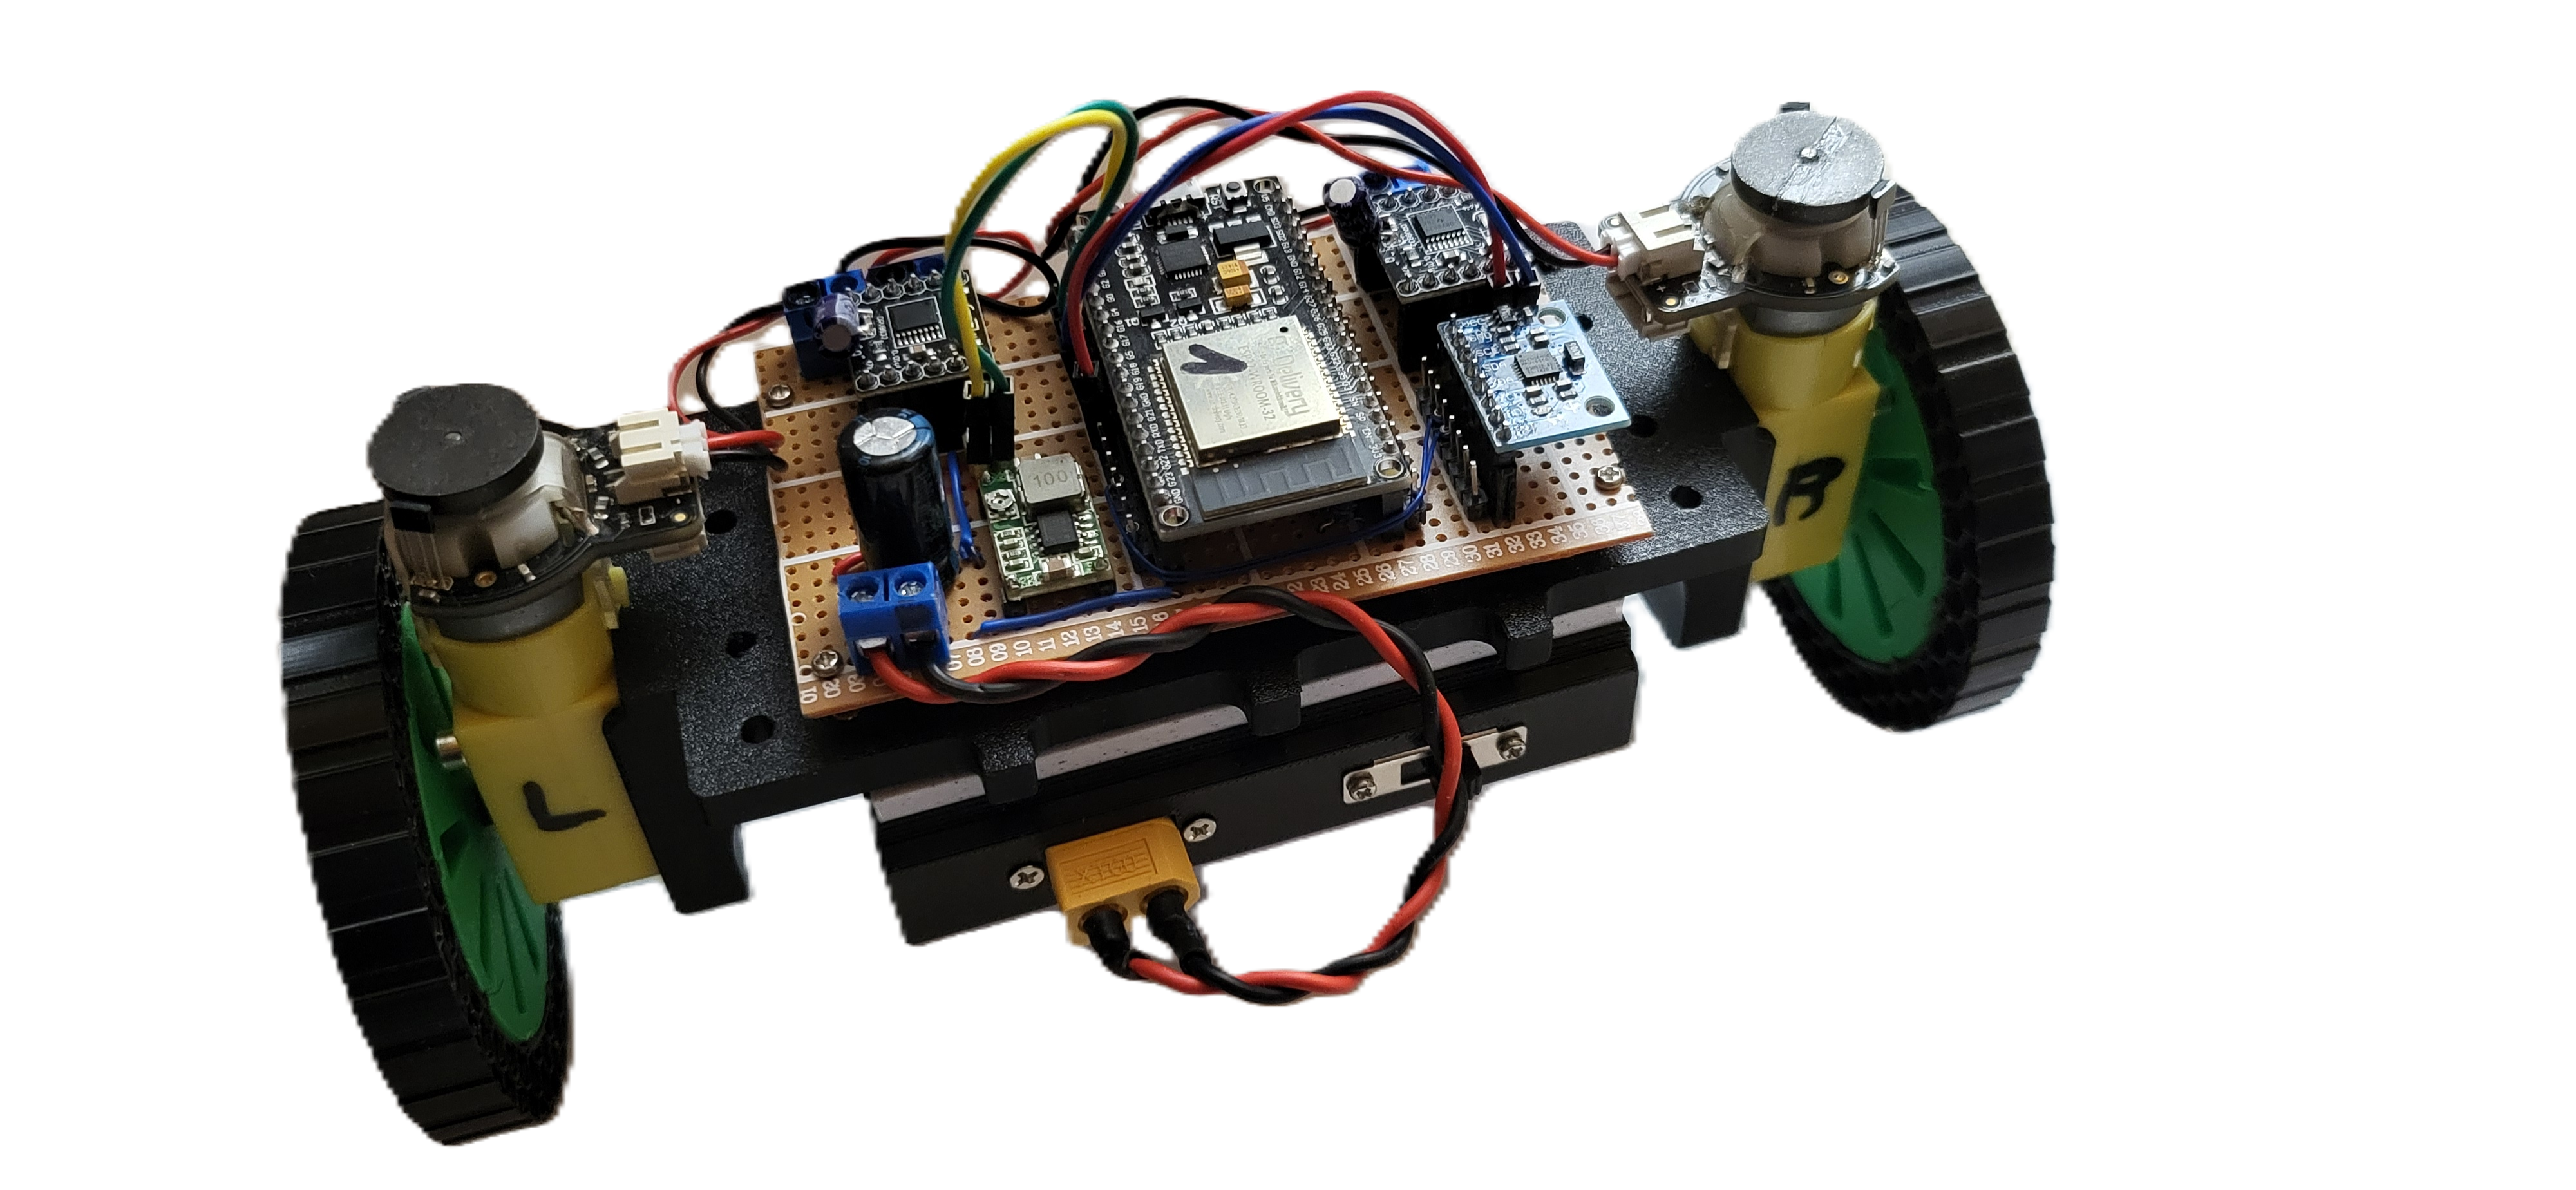
\includegraphics[width=0.7\linewidth]{figures/04_implementation/jamal_01.png}
    \caption{Robot}
\label{fig:04_robot_strucuture}
\end{figure}

The complete structure is shown in Figure \ref{fig:04_robot_strucuture}, while \ref{fig:04_tires} shows different tire designs.

\begin{figure}[h]
    \centering
    \includegraphics[width=0.7\linewidth]{figures/04_implementation/tires.jpg}
    \caption{Different tire geometries tried for the robot. Left to right for lower infill density and higher friction coefficient}
\label{fig:04_tires}
\end{figure}

During some initial tests it was found that the limited weight of the robot was not enough to ensure it stayed well connected to the ground. To reduce the loss of traction on smooth surfaces, we had to change the tire structure. Unfortunately, changing material is not really feasible, as not many flexible filaments options are available other than 95A TPU. Instead, we changed the tire density, lowering sparse infill to 15\% and eventually 8\%.
To further add flexibility, the shoulder of the tire had to be increased too, resulting in a larger diameter. Thanks to this simple solution, the tire deforms enough under torque to stay well connected to smooth tabletops.

\subsection{PID adjustments}

The PID controller parameters obtained in Chapter \ref{chap_02:modelling} are a good starting point for the real 
implementation, but due to the simplifications made in the model and the non-idealities of the real components,
it is necessary to adjust them experimentally.
After several tests, the final parameters used in the firmware are:
\begin{itemize}
    \item $K_P = 10$
    \item $K_I = 0.02$
    \item $K_D = 0.4$
\end{itemize}
These values ensure a good balancing performance, with a fast response to disturbances and minimal oscillations around the vertical position.

\subsection{Other adjustments}
Other parameters that needed to be adjust experimentally were for example the full-scale range of the accelerometer:
we experinced that setting it to $\pm 4g$ ensured a good compromise between sensitivity and range of measurement, while 
setting it to $\pm 2g$ resulted in a high noise measurement.

In order to use the robot without the need of a computer connected via USB, we inserted a simple buck converter to power the ESP32
from the batteries.
\end{chapter}
    \cleardoublepage{}

    \begin{chapter} {Conclusions}
\label{chap_05:conclusions}

In this report, we presented the design and implementation of a self-balancing robot using an ESP32 microcontroller 
and an MPU6050 IMU sensor. We modelled the system as an inverted pendulum and designed a PID controller to maintain balance. The physical implementation involved selecting appropriate hardware components,
designing a mechanical structure, and tuning the controller parameters experimentally.
The final robot successfully demonstrated the ability to balance itself and respond to disturbances, validating our modelling and control approach. 
Future work could involve exploring more advanced control strategies or implementation of a wireless interface for remote monitoring and control.

In this project we were able to apply theoretical concepts learned in class but also to gain practical
experience in analyzing and solving real-world engineering problems.

\end{chapter}
    \cleardoublepage{}

    \appendix
\chapter{MATLAB code}
\label{chap_ZZ:appendixMatlab}

In this appendix the main MATLAB code used for the modelling and controller design of the self-balancing robot is reported.

\begin{lstlisting}[language=Matlab, caption=MATLAB code for PID tuning, label=lst:ZZ_pidTuning, style=mystyle]
%% Self-balancing robot parameters

% Using stand-alone model of DC motor and inverse pendulum to derive transfer function
clc;
clearvars;
% Inverse pendulum data
% [Kg] total mass, considering also motors and battery
m = 0.1; 
% [m/s^2] gravity acceleration   
g = 9.81;   
% [m] length of the pendulum
l = 0.08;    
% [Kg*m^2] moment of inertia of inverse pendulum
J = m*l^2;  

% DC motor parameters
% [ohm] measured resistance
R = 3.5;    
% [H] estimated from comparison with similar motors
L = 50e-6;    
% [V*s] torque costant (Va_max-Ra*Ia)*1/Omega_max
KePhi = 0.336;  
% gear ratio
k_gear = 120;   

%% Transfer functions
s = tf('s');
% between torque to angle of the inverse pendulum
G_torq_ang = (1/J) *(1/(s^2 - g/l));
figure('Name', 'Transfer function of the inverse pendulum');
bode(G_ang_torq);

% between voltage to torque of the DC motor
G_volt_torq = KePhi * k_gear/(R + L*s); 
figure('Name', 'Transfer function of the DC motor');
bode(G_torq_volt);

% total transfer function
G_sys = G_volt_torq*G_torq_ang;

%% Requirements: tempo di salita e overshoot
% rise time
ts = 50e-3;
% overshoot choosen to be under a safe margin of maximum voltage of DC motors, that is 7.5V
M = 0.15;

% Crossover frequency and phase margin
fct = 2/(ts*2*pi);
pmt = 1.04 - 0.8*M;

% PID tuning options
opt = pidtuneOptions;
opt.PhaseMargin = 180*pmt/pi;

% PID controller design, with filter to reduce noise in derivative action
gi = pidtune(G_sys, 'pidf', 2*pi*fct, opt);

% Regulator transfer function
G_reg = gi.Kp + gi.Ki/s + gi.Kd*s/(1+s*gi.Tf);

fprintf('PID parameters: Kp %.4f, Ki %.4f, Kd %.4f\n', gi.Kp, gi.Ki, gi.Kd);

[Nreg, Dreg] = tfdata(G_reg, 'v'); 
margin(G_reg*G_sys);
grid on;

%% Step response of the closed loop system
G_cl = feedback(G_reg*G_sys, 1);
figure('Name', 'Step response of the closed loop system');
stepSetting = RespConfig('Amplitude', 20, 'Bias', -20);
step(G_cl, stepSetting);
title('Step response of the closed loop system');
grid on;
hold on;
ylabel("Angle (degrees)");
xlabel("Time");
fontsize(gca, 13, 'points');
\end{lstlisting}

\chapter{ESP32 code}
\label{chap_ZZ:appendixESP32}

\begin{lstlisting}[language=C++, caption=Arduino code for ESP 32, label=lst:ZZ_firmware, style=mystyle]
// Load necessary libraries
#include <Arduino.h>
#include <Wire.h>
#include <MPU6050.h>
#include <PID_v1.h>

// Define pin numbers
#define SDA_PIN 21
#define SCL_PIN 22

#define DEBUG_PIN_1 2
#define DEBUG_PIN_2 0

#define M_R_forward 18
#define M_R_backward 17
#define M_L_forward 4
#define M_L_backward 16
 
// Target angle in degrees
#define PID_REFERENCE 0
#define CRASH_TRESHOLD 60

#define CH_M_R_forward 0
#define CH_M_R_backward 1
#define CH_M_L_forward 2
#define CH_M_L_backward 3


#define ACC_FILTER_ALPHA 0.2 // LPF coefficient for ACCELEROMETER reading
#define FUSION_FILTER_ALPHA 0.98


// STATE MACHINE STATES
typedef enum{
  STATE_INIT,
  STATE_MEASURE_ANGLE,
  STATE_COMPUTE_PID,
  STATE_DRIVE_MOTORS,
  STATE_RESTART,
  STATE_CRASHED
}RobotState;

struct AccFilter{
  double  ax_f;  // ax filtered value
  double  ay_f;  // ay filtered value
  double  az_f;  // az filtered value
  double  alpha;  // filter coefficient
};

struct GyroFilter{
  double  ax_f;  // ax filtered value
  double  ay_f;  // ay filtered value
  double  az_f;  // az filtered value
  double  alpha;  // filter coefficient
};

AccFilter accFilter = {0,0,0,ACC_FILTER_ALPHA};

struct EstimatedAngle{
  double  acc;     // [deg] accelerometer estimated angle
  double  gyro;    // [deg] gyroscope estimated angle
  double  fusion;  // [deg] estimated angle using sensor fusion
  double  gyroRate; // [deg/s] gyro rate of change of the angle 
};
EstimatedAngle angle = {0.0,0.0,0.0};

// SERIAL PRINTING
struct Sample {
    double angleAcc;
    double angleGyro;
    double error;
    double control;
    double rateGyro;
};
Sample buf[512];
volatile int wptr = 0;
volatile int wptr_old = 0;

/* Define PID parameters
 Input => Measured value
 Output => Voltage applied to motor
 Setpoint => Desired value of angle, stable at 0 degrees */
 double Setpoint, Input, Output;

// PID tuning parameters

uint16_t sampleTime = 4; //sampletime in ms 
double Kp=10, Ki=0.02, Kd=0.4; //08/12/2025 15:05
// Create an MPU6050 object
MPU6050 mpu;

// Create a PID controller object
PID controller(&Input, &Output, &Setpoint, Kp, Ki, Kd, DIRECT);

// Variables for angle calculations
double pitchAcc, pitchGyro, rateGyro;

// Complementary filter
unsigned long imuFilter_lastCall=0; 

// Complementary filter parameters
double imuFilter_alpha = 0.93; // Complementary filter coefficient -> higher value gives more weight to gyroscope

// PWM definition at 8 bit
// Impostazioni PWM
const int pins[] = {M_R_forward, M_R_backward, M_L_forward, M_L_backward};
const int channels[] = {CH_M_R_forward, CH_M_R_backward, CH_M_L_forward, CH_M_L_backward};
const int freq = 100;//19531;  // Frequenza massima per 12 bit (80 MHz / 4096)
const int res = 8;

hw_timer_t *Timer0_Cfg = NULL;
portMUX_TYPE timerMux = portMUX_INITIALIZER_UNLOCKED;
volatile bool tick = false;
uint16_t time_count = 0;

RobotState currentState = STATE_INIT;

EstimatedAngle angleEstimation(EstimatedAngle previousAngle);
void motorControl(int16_t pwm);
void PIDresponse(double angle_deg);

void IRAM_ATTR Timer0_ISR(){
  portENTER_CRITICAL_ISR(&timerMux);
  tick = true;
  portEXIT_CRITICAL_ISR(&timerMux);
}


void setup() {
  
  pinMode(SDA_PIN, INPUT);
  pinMode(SCL_PIN, INPUT);
  pinMode(M_R_forward, OUTPUT);
  pinMode(M_R_backward, OUTPUT);
  pinMode(M_L_forward, OUTPUT);
  pinMode(M_L_backward, OUTPUT);
  pinMode(DEBUG_PIN_1, OUTPUT);
  pinMode(DEBUG_PIN_2, OUTPUT);

  Serial.begin(115200);
  Wire.begin();

  Serial.println("MPU6050 Initialization...");
  mpu.initialize();

  if (!mpu.testConnection()) {
    Serial.println("Unable to connect to MPU6050!");
    while (1);
  }
  Serial.println("MPU6050 connected succesfully!");

  mpu.setFullScaleGyroRange(MPU6050_GYRO_FS_250); // set gyro range to maximum 250 degrees (best resolution)
  mpu.setFullScaleAccelRange(MPU6050_ACCEL_FS_4); // set accelerometer range to maximum 4g

  mpu.CalibrateAccel(6);  // 6 samples for calibration
  mpu.CalibrateGyro(6);

  Serial.println("Initial Calibration Completed!");
  mpu.PrintActiveOffsets();  // Mostra gli offset calcolati


  // Imposta il setpoint iniziale
  Setpoint = PID_REFERENCE; // Target angle in degrees
  controller.SetMode(AUTOMATIC); // Attiva il PID controller

  //calibrateGyroBias();
  Serial.println("Regulator Setup Completed!");

  // Configura i canali PWM
  for (int i = 0; i < 4; i++) {
    ledcSetup(channels[i], freq, res);
    ledcAttachPin(pins[i], channels[i]);
  }

  Timer0_Cfg = timerBegin(0, 80, true); // 80e6/80 = 1e6 => 1 tick = 1 us
  timerAttachInterrupt(Timer0_Cfg, &Timer0_ISR, true);
  timerAlarmWrite(Timer0_Cfg, 1000, true); //1000*1us = 1ms
  timerAlarmEnable(Timer0_Cfg);

  delay(1000);

  currentState = STATE_MEASURE_ANGLE;

}

void loop() {
  if(tick == true){
    portENTER_CRITICAL(&timerMux);
    tick = false;
    portEXIT_CRITICAL(&timerMux);

    //if(time_count == 10){
      time_count = 0;
      switch(currentState){
        case STATE_MEASURE_ANGLE:{
          
          angle=angleEstimation(angle);
          if(angle.acc>CRASH_TRESHOLD || angle.acc<-CRASH_TRESHOLD){
            currentState = STATE_CRASHED;
          }else{
            currentState = STATE_COMPUTE_PID;
          }
          digitalWrite(DEBUG_PIN_1, 1);
          break;
        }
        case STATE_COMPUTE_PID:{
          PIDresponse(angle.fusion);
          currentState = STATE_DRIVE_MOTORS;
          break;
        }
        case STATE_DRIVE_MOTORS:{
          motorControl(Output);
          digitalWrite(DEBUG_PIN_1, 0);
          buf[wptr] = {angle.acc, angle.gyro, angle.fusion, Output, angle.gyroRate}; // buffer for serial print
          wptr = (wptr + 1) % 512;
          currentState = STATE_MEASURE_ANGLE;
          break;
        }
        case STATE_CRASHED:{
          motorControl(0);
          PIDresponse(0);
          buf[wptr] = {angle.acc, angle.gyro, angle.fusion, Output, angle.gyroRate}; // buffer for serial print
          wptr = (wptr + 1) % 512;
          //Serial.println("\nCRASHED!\n");
          currentState = STATE_MEASURE_ANGLE;
          break;
        }
      }
    }
    //Serial.println("Angle: " + String(angle) + " Pitch Acc " + String(pitchAcc) + " Pitch Gyro " + String(pitchGyro) + " PID Output "+ String(Output)+",");
    //Serial.println(String(angle) +","+ String(pitchAcc) +","+ String(pitchGyro) +","+ String(Output)+" ");

    if((wptr != wptr_old) && (wptr%10==0)){
      Serial.print((int16_t)(buf[wptr].angleAcc));
      Serial.print(",");
      Serial.print((int16_t)(buf[wptr].angleGyro));
      Serial.print(",");
      Serial.print((int16_t)(buf[wptr].error));
      Serial.print(",");
      Serial.print((int16_t)(buf[wptr].control));
      Serial.print(",");
      Serial.print((int16_t)(buf[wptr].rateGyro));
      Serial.print("\n");
      wptr_old = wptr;
    }

    //time_count++;
  }
//}

// Function to estimate angle using complementary filter
EstimatedAngle angleEstimation(EstimatedAngle previousAngle){
  int16_t ax=0, ay=0, az=0, gx=0, gy=0, gz=0;
  double ax_d=0, ay_d=0, az_d=0;
  double gyroRate = 0;

  EstimatedAngle measAngle;
  mpu.getMotion6(&ax, &ay, &az, &gx, &gy, &gz); // Legge i dati grezzi da MPU6050

  ax_d = (double)ax * 0.002394202; // (9.8/4096) for 8g acceleration range 
  ay_d = (double)ay * 0.002394202;
  az_d = (double)az * 0.002394202;
  
  accFilter.ax_f += accFilter.alpha * (ax_d - accFilter.ax_f);
  accFilter.ay_f += accFilter.alpha * (ay_d - accFilter.ay_f);
  accFilter.az_f += accFilter.alpha * (az_d - accFilter.az_f);

  // Estimation pitch angle (y-axis) accelerometer
  measAngle.acc = atan2(ay_d, az_d)*(360/PI); // angle estimated from accelerometer (FILTERED)
  
  // Estimation pitch angle (y-axis) gyroscope
  gyroRate = (double)gx * (1.0/131); // [deg/s]

  // This block finds the elapsed time between the current and the previous function call to determine the integration interval 
  unsigned long imuFilter_now = micros();
  double imuFilter_dt=0;
  if(imuFilter_lastCall == 0){
    imuFilter_dt = 1e-3;
  }else{
    imuFilter_dt = (double)(imuFilter_now - imuFilter_lastCall) / 1e6;
  }
  imuFilter_lastCall = imuFilter_now;

  measAngle.gyro = previousAngle.gyro + gyroRate * imuFilter_dt; // [deg] angle estimated from gyroscope rate integrated over time

  // Complementary filter to combine accelerometer and gyroscope data
  measAngle.fusion = FUSION_FILTER_ALPHA * (previousAngle.fusion + gyroRate * imuFilter_dt) + (1 - FUSION_FILTER_ALPHA) * measAngle.acc;  //dt =0.03 max limit for oscillations 
  measAngle.gyroRate = gyroRate;
  return measAngle;
}

// PID response function
void PIDresponse(double angle_deg){
// Input of PID will be the y-axis angle
  Input = angle_deg; //* PI/180; // in radians
  controller.Compute(); // Calcola il nuovo output del PID
  controller.SetOutputLimits(-255, 255);//(-4095, 4095); // Limita l'output tra -4095 e 4095 (12 bit)
  controller.SetSampleTime(sampleTime);
}

 // Control motors based on PID output
void motorControl(int16_t pwm){

  if (Output > 0) {
    // Move forward
    ledcWrite(CH_M_R_forward, pwm);//analogWrite(M_R_forward, Output);
    ledcWrite(CH_M_R_backward, 0);
    ledcWrite(CH_M_L_forward, pwm);
    ledcWrite(CH_M_L_backward, 0);
  } 
  else if (Output < 0) {
    // Move backward
    ledcWrite(CH_M_R_forward, 0);
    ledcWrite(CH_M_R_backward, -pwm);
    ledcWrite(CH_M_L_forward, 0);
    ledcWrite(CH_M_L_backward, -pwm);
  } 
  else {
    // Stop
    ledcWrite(CH_M_R_forward, 0);
    ledcWrite(CH_M_R_backward, 0);
    ledcWrite(CH_M_L_forward, 0);
    ledcWrite(CH_M_L_backward, 0);
  }
}
\end{lstlisting}

    \cleardoublepage{}
\end{document}